\section{Chapter 1} 
I didn't (and probably won't be) taking lecture notes during class so instead I'll be taking notes from Pitman here.

\begin{definition}[]
    An \textbf{outcome space} $\Omega$ is a set of all possible outcomes. \textbf{Events} (denoted $A$) are subsets of the outcome space and a \textbf{probability} $P$ is a function of such events to $[0,1]$.
\end{definition}
\begin{example}
    If a crowd has 1000 people, 700 women and 300 men, let $\Omega=\{ 1000 \ \text{people} \} $, $A= \{ \text{women} \} $ where $|A|=700$, then $P(A)=\frac{700}{1000}=0.7$.
\end{example}
In general, if all outcomes of $\Omega$ are equally likely, then $P(A)= \frac{|A|}{| \Omega|}  $.

\begin{example}
    Suppose there is a box of 100 tickets marked $1,2,3, \cdots ,100$ ($\Omega=\{1,\cdots ,100\} $). If tickets are drawn at random, here are some events and their probability:
    \begin{itemize}
    \setlength\itemsep{-.2em}
\item The number drawn having one digit is represented by $A= \{1,\cdots ,9\} $, then $|A|=9$ and $P(A)=\frac{9}{100}=0.09$.
\item The number drawn having two digits is represented by $A= \{10,\cdots ,99\} $ where $|A|=90$, so $P(A)= \frac{90}{100}=0.9$.
\item The number drawn being $\leq k$ is represented by $A=\{1,\cdots ,k\} $ where $|A|=k$, so $P(A)=\frac{k}{100}$.
\item The number drawn being $>k$ is represented by $A=\{k+1,\cdots ,100\} $ where $|A|=100-k$, so $P(A)=\frac{100-k}{100}$.
\item The number drawn having digits summing to 3 is represented by $A=\{3,12,21,30\} $, so $|A|=4$ and $P(A)=\frac{4}{100}=0.04$.
    \end{itemize}
\end{example}

\begin{example}
    Roll two $n$-sided die with faces $1,2, \cdots ,n$, where $n \geq 4$. To find the chance the sum is 5, note that there are $n^2$ possible pairs, but only four possible pairs with sum 5. So $P(\text{sum is} \ 5)=4 /n^2$. 

    To fine the chance that the second number is greater than the first, this is all pairs above the diagonal so summing $1+2+ \cdots +(n-1)$ gives $\frac{n(n-1)}{2}$.
\end{example}
\subsection{Combinatorics}

Digression on elementary combinatorics. If we have a set of $n$ elements, and we want to list the number of length $k$ lists without repetition, we start by multiplying $n$ by $(n-1)$ (since we can't use the element from earlier), then $(n-2),(n-3)\cdots $ a total of $k$ times, one for each slot. So the formula is \[
    n(n-1)(n-2)\cdots (n-k+1)= \frac{n!}{(n-k)!}.
\] To find the value of ${n \choose k} $, the number of length $k$ subsets of a set of cardinality $n$, first note that for $k=0$ we have ${n \choose k} =1$, and if $k<0$ or $k>n$, then ${n \choose k} =0 $. Now given a subset $ \{1,\cdots ,k\} $, there are $k!$ different ways of permuting these elements, therefore \[
| \{\text{permutations of} \ k\} | \cdot | \{ \text{subsets of length} \ k \} = | \{ \text{unique lists of length} \ k\}|. 
\] However, we know the values of the first factor on the left and the RHS, and the second factor is just ${n\choose k} $. So plug everything in to get  \[
k! \cdot {n \choose k} = \frac{n!}{(n-k)!} \implies {n \choose k} = \frac{n!}{k!(n-k)!}.
\] Note that ${n \choose k} ={n \choose n-k} $ since choosing $k$ elements is the same thing as choosing $n-k$ elements to be left behind. 

Furthermore, we have the identity 
\[
{n+1 \choose k} = {n \choose k-1} +{n \choose k}.
\] 
 To think about this, choosing length $k$ subsets of $\{1,\cdots ,n+1\} $ is the same as choosing length $k$ subsets containing an element $a \in \{1,\cdots ,n+1\} $ and choosing length $k$ subsets containing everything except $a$. In the first case, we are only choosing length $k-1$ subsets out of a set of $n$ elements, since $a$ is fixed, so this gives us ${n \choose k-1} $. For the second case, we remove $a$ from the set of outcomes giving us a set of order $n$, therefore the value is ${n\choose k} $. Adding gives the expected result ${n+1 \choose k} ={n \choose k-1} +{n \choose k} $. 

 \begin{figure}[h]
\centering
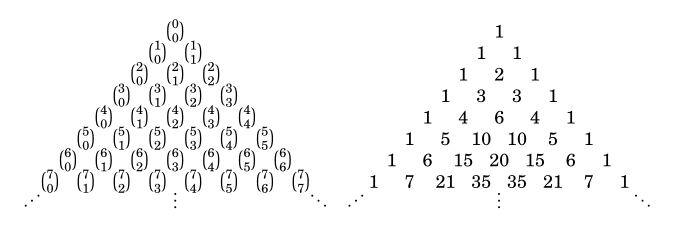
\includegraphics[width=0.7\linewidth]{figures/pascals_triangle.png}
\caption{Pascal's triangle.}
\label{pascal}
\end{figure}

Consider Pascal's triangle as in \cref{pascal}. The $n$th row consists of the entries ${n\choose 0} ,{n\choose 1} ,\cdots ,{n\choose n} $. The $k$th entry of the $(n+1)$th row, or ${n+1\choose k} $, is the sum of the two elements above it in the triangle, or ${n\choose k-1} +{n\choose k} $, which agrees with our formula.

Furthermore, note that the coefficients of the expansion $(x+y)^3=x^3+3x^2y+3xy^2+y^3$ agree with the 3rd row of Pascal's triangle. This can be generalized in the following theorem.
\begin{namedthm}{Binomial Theorem} 
   If $n \in \N$, then \[
       (x+y)^n  = {n\choose 0} x^n +{n\choose 1} x^{n-1}y+{n\choose 2} x^{n-2}y^2 + \cdots + {n\choose n-1} xy^{n-1}+{n\choose n} y^n .
   \]  
\end{namedthm}

\subsection{Inclusion-Exclusion}
To avoid overcounting, note that $|A \cup B|=|A|+|B|-|A\cap B|$. This formula is sometimes called \textbf{inclusion-exclusion} because we \emph{include} elements of $A \cup B$ twice when adding together $|A|+|B|$, then \emph{exclude} them by subtracting $|A \cap B|$.We can deduce that if $|A \cup B|=|A|+|B|$, then it must be the case that $A\cap B=\O$.

There is a generalization of this for three sets $A,B,C$, which says that \[
|A \cup B\cup C|=|A|+|B|+|C| -|A\cap B|-|A\cap C|-|B\cap C|+|A\cap B\cap C|.
\] We add $|A \cap B\cap C|$ at the end because we over count it three times but subtract it three times, with a net addition of zero. So we add it back in at the end. The principle that $A\cap B=\O$ if $|A \cup B|=|A|+|B|$ also generalizes: if we have a collection of sets $\{A_i \} _{i \in I}$ with $A_i  \cap A_j =\O$ for $i, j \in I$, $i\neq j$, then $|A_1 \cup  \cdots \cup A_n |=|A_1|+ \cdots + |A_n |$.

\begin{example}
    A 3 card hand is dealt from a standard 52 card deck. How many different hands are there with all 3 cards red or all 3 cards face cards?
\end{example}
\begin{solution}
    The goal is to count $|A \cup B|$ where $A=\{ \text{3 card hands, red} \} $ and $B= \{\text{3 card hands, face} \} $. There are are 26 red cards so selecting three card hands from here gives $|A|= {26 \choose 3} $. There are 12 royals so $|B|={12\choose 3} $. There are 6 royal face cards so $|A \cap B|={6\choose 3} $. By inclusion-exclusion, \[
        |A \cup B|=|A|+|B|-|A \cap B|= \frac{26!}{(26-3)!3!}+ \frac{12!}{(12-3)!3!}- \frac{6!}{(6-3)!3!}=2800.\qedhere
    \] 
\end{solution}
\begin{example}
    How many 7-digit binary strings (0100110, 0101001, etc) have an odd number of 1's?
\end{example}
\begin{solution}
    If $A$ is the set of 7-digit binary strings with an odd number of 1's, note that $A$ consists of the set of binary strings with one 1, three 1's, five 1's, and seven 1's. All of these are disjoint so all we need to do is count these subsets and add. A string with $n$ 1's is made by choosing three positions from seven options, and since value doesn't matter the number of strings is ${7\choose 3} $. By this logic, 
    \[
    |A|={7\choose 7} +{7\choose 5} +{7\choose 3} +{7\choose 1} =64.\qedhere
    \] 
\end{solution}

\subsection{Odds}
Given equally likely outcomes, \textbf{odds in favor}  of $A$ is a ratio of the number of ways $A$ could happen to the number of ways $A$ does not happen. \textbf{Odds against}  $A$ give the inverse ratio. Gamblers deal with \textbf{payoff odds}, offered in a betting contract. If the payoff odds against $A$ are 10 to 1, and you stake $\$1$,  we say $\$1$ is \emph{your stake}, the $\$10$ is the \emph{casino's stake}, and the $\$11$ is the \emph{total stake}.

\begin{namedthing}{The Fair Odds Rule} 
    In a fair bet, the payoff odds equal the chance odds. That is, in a fair bet on an event $A$, the ratio of your stake to the casino's stake should be the ratio of probabilites  $P(A)$ to $1-P(A)$.
\end{namedthing}

\subsection{Interpretations}
The \textbf{frequency interpretation} is where probabilities are understood as mathematically convenient approximations to long-run relative frequencies. The \textbf{subjective interpretation} is when probabilities express the \emph{opinion} of some individual on how certain an event is to occur. A \textbf{relative frequency} is a proportion measuring how often something occurs in a sequence of observations, or \textbf{trials}. If $A$ happens $m$ times in $n$ trials, then $m /n$ is the relative frequency of $A$.

In the frequency interpretation, the probability of an event $A$ is the estimated relative frequency of $A$ in a large number of trials. Let $P_n (A)$ be the relative frequency of $A$ in $n$ trials. It should be the case that \[
    P_n (A) \approx P(A) \quad \text{for large} \ n.
\] The \textbf{law of large numbers} makes this precise by saying that $\lim _{n \to \infty}P_n (A)=P(A)$.

Sometimes it isn't practical to give probabilities in terms of trials, like your probability of surviving an operation. Some sort of intuitive judgement of the situation leads to the notion of \textbf{subjective probabilities}, or \emph{probabilistic opinions,} or \emph{degrees of belief}. For example:
\begin{itemize}
\setlength\itemsep{-.2em}
    \item It is unlikely that there will be an earthquake in Berkeley next year.
    \item If I toss a coin once, the probability that it will land heads is $\sfrac{1}{2}$.
    \item The chance of rain tomorrow is $30\%$.
\end{itemize}
These statements are hard to interpret objectively, but make sense. To interpret them as probabilities, it is best to view them as subjective opinions. The subjective interpretation gives insight into probability theory, for example conditional probability which changes as you acquire new information or data.

\subsection{Distributions}
Events are subsets, so logical relations between events are translated into the language of sets. For example, if $C$ is the event where events $A,B$ both occur, then $C=A \cap B.$ Recall partitions are a collection of subsets such that $B = \bigcup_{i \in I} B_i $, $B_i \cap B_j =\O$ for $i,j \in I$.

\begin{namedthing}{Rules of proportion and probability} 
\hspace{0.2em} 

    \begin{itemize}
    \setlength\itemsep{-.2em}
\item \textbf{Non-negative}: $P(B) \geq 0$ 
\item \textbf{Addition}: If $B_1,B_2,\cdots ,B_n $ is a partition of $B$, then \[
        P(B)=\sum _i P(B_i ).
    \] \item \textbf{Total one}: $P(\Omega)=1$
    \end{itemize}
    A \textbf{distribution} over $\Omega$ is a function mapping subsets of $\Omega$ to a probability (satisfying the above rules).    
\end{namedthing}
Some useful rules of probability: the \textbf{complement rule} says that $P(\sim A)=P(A^{c})=1-P(A)$. This is because $\Omega$ is partitioned into $A$ and $A^{c}$, so $P(\Omega)=1=P(A)+P(A^c)$. This implies that $P(\O)=0$, and $P(A)=1-P(A^{c}),P(A) \geq 0$ ($P(A)\leq 1$, or probabilites of events are between 0 and 1). The \textbf{difference rule} says that if $P(A) \implies P(B)$, then $P(A) \leq P(B)$, and \[
    P(B \ \text{and not} \ A)=P(B\cap A^{c})=P(B)-P(A).
\] To see this, note that $A \subseteq B$, so $P(B)=P(A)+P(B \cap A^{c})$. Similarly, \textbf{inclusion-exclusion} tells is that $P(A \cup B)=P(A)+P(B)-P(A \cap B)$.

\begin{example}
In a certain population, $10\%$ of the people are rich, $5\%$ are famous, and $3\%$ are rich and famous.    
\begin{itemize}
\setlength\itemsep{-.2em}
    \item The chances of a person not being rich is $P(\text{not rich} )=100\%-P( \text{rich} )=90\%$.
    \item The chance of a person being rich but not famous is $P(\text{rich} \ \cap \sim \text{famous} )=10\%-3\%=7\%$.
    \item The chance of a person being either rich or famous is $P(\text{rich} \ \cup \ \text{famous} )=10\%+5\%-3\%=12\%$.
\end{itemize}
\end{example}
For a \textbf{normed distribution}, consider some event $A$ where it makes sense to consider $P(A)$ (eg a biased coin toss). Define an outcome (the \textbf{indicator} of $A$) to be 1 if $A$ occurs and 0 otherwise, called the \textbf{Bernoulli} ($p$) \textbf{distribution}  for $p=P(A)$.

Sometimes named distributions have parameters, constants appearing in the formula that affecting its shape and properties. Typically parameters are subject to constraints like non-negativity so that things are well-defined. In this case, $p$ is the parameter of the Bernoulli $(p)$ distribution.

{\color{red}todo:uniform, empirical distribution} 

\subsection{Conditional probability and independence}
Say you bet on 2 or more heads appearing in 3 fair coin tosses ($A$): then the overall \emph{unconditional} probability of $A$ is $P(A)=\frac{1}{2}$. However, if the first toss lands heads ($H$), then the probability of a heads in the next two tosses becomes $\frac{3}{4}$. So the conditional probability of $A$ given $H$ is $\frac{3}{4}$, or  $P(A \mid H)=\frac{3}{4}$. We can interpret this by saying $H$ occurs four ways, and three of those ways makes $A$ occur. This is precisely the intersection $A \cap H$. Similarly, $P(A \mid H^{c})=\frac{1}{4}$.

\begin{namedthing}{Counting formula for $P(A\mid B)$} 
    For a finite set $\Omega$ of equally likely outcomes, and events $A,B$, the \textbf{conditional probability} of $A$ given $B$ is \[
        P(A \mid B)= \frac{|A \cap B|}{|B|}.
    \] 
\end{namedthing}
Rearrage to get the \textbf{multiplication rule}: $P(A \cap B)=P(A \mid B)P(B)$. This is how we get tree diagrams: the first branch is $P(B)$ and the second is $P(A\mid B)$. For events $A,B$, the overall probability $P(A)$ is the average of the two conditional probabilities $P(A \mid B)$ and $P(A \mid B^{c})$ with weightcs $P(B)$ and $P(B^{c})$: \[
    P(A)=P(A \mid B)P(B)+P(A \mid B^{c})P(B^{c}).
\] This corresponds to the sum of paths in a tree diagram. If the family  $\{B_i \}$ forms a partition of the outcome space $\Omega$, for any event $A$ the events $A \cap B_1, \cdots ,A\cap B_n $ form a partition of $A$, so \[
P(A)+P(A \cap B_1) + \cdots + P(AB_n )
\] by the addition rule. Applying the multiplication rule gives \[
P(A)= P(A \mid B_1)P(B_1) + \cdots + P(A\mid B_n )P(B_n ).
\] This is the \textbf{rule of average conditional probabilities}. 

Suppose the probability of $A$ doesn't depend on $B$, in other words, $P(A \mid B)=P(A \mid B^{c})=p$. Then \[
    P(A)=P(A\mid B)P(B)+P(A\mid B^{c})P(B^{c})=p P(B)+p P(B ^{c})=p.
\] Note that $P(A \mid B)=P(A)$ for independent events, and the formula $P(A \mid B)= P(A \cap B) / P(B)$ gives us the \textbf{multiplication rule for independent events}: $P(A \cap B)=P(A)P(B)$. As an example, since $A $ splits into $A \cap B^{c}$ and $A \cap B$, 
\begin{align*}
    P(A\cap B^{c})&= P(A)-P(A \cap B)\\
                  &=P(A)-P(A)P(B) \quad \text{assuming the multiplication rule} \\
                  &=P(A)(1-P(B))\\
                  &=P(A)P(B^{c}).
\end{align*}So the multiplication rule works for $B^{c}$ as well as $A^{c}$ (by the same logic).

\subsection{Bayes' Theorem}
We say two events are \textbf{mutually exclusive} if $P(A)+P(B)=P(A \cup B)$. Say we have some mutually exclusive events $B_i $, whichever one occured is unknown. We observe the result of $A$, which depends on $B_i $, and we want to calculate the probabilities of $B_i $ given $A$ (\emph{posterior probabilities}), in terms of 
\begin{enumerate}[label=(\roman*)]
\setlength\itemsep{-.2em}
    \item the unconditional probabilities $P(B_i )$ (called \emph{prior probabilities});
    \item the conditional probabilities $P(A \mid B_i )$ (called \emph{likelihoods}).
\end{enumerate}In general, \[
P(B_i  \mid A)= \frac{P(A \cap B_i )}{P(A)}= \frac{P(A \mid B_i )P(B_i )}{P(A)},
\] by the multiplication rule where \[
P(A)=\sum _i^n  P(A \mid B_i )P(B_i )
\] by the rule of average conditional probabilities.
\begin{namedthm}{Bayes' Theorem} 
    For a partition $B_1 ,\cdots ,B_n $ of all possible outcomes, \[
        P(B_i \mid A)= \frac{P(A \mid B_i )P(B_i )}{\sum _i ^n  P(A \mid B_i )P(B_i )}.
    \]  
\end{namedthm}
If the prior odds ratios are written as $R_i $ to $R_j $, and the likelihood ratios are written as say $L_i $ to $L_j $, then the \textbf{posterior odds ratios} $P(B_i  \mid A)$ to $P(B_j  \mid A)$ are simply $R_i L_i $ to $R_j L_j $, and \[
    P(B_i  \mid A) = \frac{R_i L_i }{\sum _i ^n R_i }.
\] This is \textbf{Bayes' rule for odds}: posterior odds $=$ prior odds $\times $ likelihoods.

\subsection{Sequences of events}
To calculate $P(A \cap B\cap C)$, we have \[
    P(A \cap B\cap C)= P(A \cap B)P(C \mid A \cap B)=P(A)P(B \mid A)P(C \mid A \cap B).
\] Extend this argument inductively to get the probability of $A_i $ events occuring, the \textbf{multiplication rule for} $\mathbf n$ \textbf{events}: \[
P(A_1 \cap  A_2 \cap A_3 \cap  \cdots \cap A_n )=P(A_1)P(A_2 \mid A_1)P(A_3\mid A_1 \cap A_2) \cdots P(A_n \mid A_1\cap A_2 \cap \cdots \cap A_{n-1}).
\]In other words,
\[
    P \left( \bigcap_{i=1} ^n A_i \right)= \prod _{i=1} ^n  P\left( A_i  \,\Big|\  \prod _{j=1}^{i-1}A_i   \right) .
\] 
\subsection{Independence}

We say events $A,B,C$ are \textbf{independent} if $P(B \mid A)=P(B \mid A ^c)=P(B)$, and \[
    P(C \mid A \cap B)= P(C \mid A^c \cap B) = P(C \mid A \cap B^c)=P(C \mid  A^c B^c)=P(C).
\] This gives us the \textbf{multiplication rule for three independent events:} $P(A \cap B \cap C)=P(A)P(B)P(C)$.
